\documentclass{article}

\usepackage{arxiv}

\usepackage[utf8]{inputenc} % allow utf-8 input
\usepackage[T1]{fontenc}    % use 8-bit T1 fonts
\usepackage{hyperref}       % hyperlinks
\usepackage{url}            % simple URL typesetting
\usepackage{booktabs}       % professional-quality tables
\usepackage{amsfonts}       % blackboard math symbols
\usepackage{nicefrac}       % compact symbols for 1/2, etc.
\usepackage{microtype}      % microtypography
\usepackage{lipsum}
\usepackage{graphicx}
\graphicspath{ {./images/} }

\usepackage{float}
\usepackage{tikz}
\usetikzlibrary{arrows.meta}

\usepackage{xcolor}
\title{Do emotions affect LLMs' performance on question-answering tasks?}


\author{
  Fabio Cirullo \\
  Department of Computer Science \\
  University of Bari Aldo Moro \\
  Bari, Italy \\
  \texttt{f.cirullo@studenti.uniba.it} \\
}

\usepackage{fancyhdr}
\rhead{}

\begin{document}
\renewcommand{\today}{}
\maketitle

\begin{abstract}
Activation steering changes the behaviour of large language models (LLMs) at inference time by adding a direction to their residual stream. This technique can also be used to induce emotions, but it is not clear how it affects the model’s factual knowledge and simple logical reasoning. This work investigates whether, and at which depth, emotion steering makes the model hallucinate. Difference-of-means steering vectors are computed for ten emotions in three instruction-tuned models (Qwen2.5-7B, Llama-3.1-8B and Qwen3.8-27B), with candidate layers chosen through linear probes. For each emotion and layer, the steering strength is tuned on free generation, picking the strongest value at which the emotion clearly shows without breaking the text. The hallucination rate on BeliefBankFacts and BeliefBankConstraints is then compared with and without steering. Steering at intermediate layers increases the hallucination rate, often reducing them to a constant ``yes'' or ``no'', regardless of the statement, while at deeper layers, emotions remain visible and factual answers stay mostly intact. These results suggest that, similarly to humans, an LLM induced into an emotional state may struggle to recall facts or make simple inferences.
\end{abstract}

\section{Introduction}
In Large Language Models (LLMs), high-level concepts (such as sentiment, truthfulness, or refusal) are represented by approximately linear directions in their internal activations~\cite{park2024linearrep}. As a result, activation steering becomes possible: the addition of a vector to the residual stream of the chosen layer during inference steers the model towards the desired behaviour without fine-tuning or prompt changes~\cite{turner2024steeract}. This method does not require updating the model's weights, but only collecting activations on a set of examples. For this reason, it is widely used both in research on concept representation in LLMs and as a way to control the output.

Among the concepts that can be steered, emotions are of particular interest: controlling the emotional tone of a model is valuable for empathetic conversational agents~\cite{rashkin2019empathetic, zhou2018emotionalchat} or role-playing characters that need to adopt an appropriate style~\cite{chen2024persona}. However, this approach is not precise: the vector is added to a representation that the model also uses for every other computation, including recalling learned facts and making simple logical inferences. If making a model happy or sad changes its ability to retrieve the facts or to reason about them, emotion steering would become a trade-off between style and reliability, which would be a serious problem in most practical applications. Before it can be used safely, it is worth knowing whether this trade-off actually exists and, if it does, where in the model it appears.


Previous work has shown that steering vectors can control behaviours such as sycophancy and refusal~\cite{panickssery2024steerllama2} or character traits~\cite{chen2025personavectors}, and has started to study their side effects, finding that steering one concept can also shift others~\cite{bhandari-etal-2026-personality}. These studies, consider the side effects of steering on other traits or on general benchmarks; therefore it remains unclear whether steering a model towards an emotion changes its answers to factual and logical questions. Also, a single steering strength is often used for all concepts: this makes it difficult to tell whether an increase in hallucinations comes from the chosen emotion or simply from a strength so high that it breaks the model. This work addresses these gaps by studying how emotion steering at different depths affects factual recall and simple logical reasoning, with a strength calibrated for each emotion and layer.

The study is guided by three research questions:    
\begin{itemize}
  \item \textbf{RQ1}: which layers represent emotions linearly, and are therefore good candidates for steering?
  \item \textbf{RQ2}: for each emotion and layer, which steering strength makes the emotion clearly visible in the generated text without breaking it?
  \item \textbf{RQ3}: how does emotion steering at different depths affect the model's answers to factual questions and simple logical inferences?
\end{itemize}

\section{Related Work}
Earlier work has already looked at the side effects of steering. Contrastive Activation Addition (CAA)~\cite{panickssery2024steerllama2} computes the steering vector as the mean difference between the activations of positive and negative examples of a behaviour. In Llama~2, this technique changes behaviours like sycophancy and refusal, with only a small loss in overall performance. The results, however, vary greatly from layer to layer.

The Selective Steering method~\cite{dang2026selectivesteer} is based on choosing the layer where the activations of the two classes are well separated. In this work, the layer selection is similar since the candidate layers are chosen using linear probes. Instead of using the layer with the widest separation, steering is applied at multiple depths and the results are compared.

Steering has also been used for affective and personality-related concepts. Sentiment is represented as a single linear direction with a causal effect on the model's behaviour~\cite{tigges2023linearrep}; persona vectors~\cite{chen2025personavectors} apply steering to character traits such as evil, sycophancy, and a tendency to hallucinate. Furthermore, steering a single trait can also modify other traits: when one of the Big Five personality traits is steered, the others change as well, even if the directions are made orthogonal~\cite{bhandari-etal-2026-personality}.

Other work has applied steering to reduce hallucinations. Adaptive Activation Steering~\cite{wang2024act} shifts activations in a truthful direction during inference: the strength of the intervention is adapted to each activation, and different vectors are used for different types of hallucinations.

The effect of emotions on reasoning has long been studied in humans. Emotional content tends to impair logical reasoning compared to neutral content~\cite{blanchette2004reasoning}, and the emotional state of the reasoner has a similar effect: participants in a negative mood perform worse than those in a positive mood, but both are outperformed by participants in a neutral mood~\cite{jung2014emotions}. A similar effect has been observed in LLMs, which are less accurate on mathematically identical problems when these are framed emotionally rather than neutrally~\cite{dokme2026temper}.

Unlike the cited works, in this work ten specific emotions are steered and the resulting effects are measured on factual knowledge and simple inferences, using facts and constraints from BeliefBank~\cite{kassner2021beliefbank}.

\section{Materials}

\subsection{Emotion data}
Emotion directions were computed from EmpatheticDialogues~\cite{rashkin2019empathetic}, a dataset describing various situations in the form of first-person sentences. Each situation is labeled with the emotion felt by the person who experienced it (e.g.\ \textit{``One year during christmas, i did not get a single gift. It was a rough day for me.''}, labeled as \textit{sad}). The dataset used in this work is a reduced version of EmpatheticDialogues, available on HuggingFace~\cite{bdotloh2023edcontexts}, containing only the descriptions of the situations and their corresponding emotions, without the dialogues. The dataset includes 32 emotion labels in total. Out of these, a subset of ten emotions considered the most interesting for this study was deliberately selected: \textit{afraid}, \textit{angry}, \textit{annoyed}, \textit{anxious}, \textit{ashamed}, \textit{content}, \textit{devastated}, \textit{joyful}, \textit{sad} and \textit{trusting}. This set contains both positive and negative emotions, and some of these form pairs of similar emotions with different intensities (e.g.\ \textit{annoyed}/\textit{angry} and \textit{sad}/\textit{devastated}), while other labels, such as \textit{nostalgic}, \textit{prepared} or \textit{anticipating}, which do not fully represent an emotion, were discarded.

\subsection{Knowledge and reasoning data}
\label{sec:materials_knowledge}
The effect of steering on factual knowledge was measured on BeliefBank~\cite{kassner2021beliefbank}, a dataset containing simple statements about approximately 85 common entities, such as animals and plants. Each statement has a yes/no label, assigned by the dataset's authors, indicating whether it is true. Two versions of BeliefBank were used.

BeliefBank Facts (BBF) was used to measure factual errors. Each instance in the dataset is a short declarative sentence about a single entity (e.g.\ \textit{``an albatross is a bird.''}, \textit{yes}; \textit{``a frog is a salad.''}, \textit{no}). For each original instance, there also exists a negated version with the opposite label (e.g.\ \textit{``a dolphin is not an action.''}, \textit{yes}). This keeps the classes balanced and includes negated statements in the evaluation. In total, BBF contains 27{,}416 instances, of which 13{,}708 are labeled yes and 13{,}708 no.

BeliefBank Constraints (BBC) was used to test knowledge of relationships between concepts. Each instance, written by the dataset authors, represents relationships between concepts that can be implications (\textit{if A then B}, e.g.\ \textit{``If an albatross is a tree, then an albatross is a living thing''}, \textit{yes}) or mutual exclusions (\textit{``If A, then not B''}). Often, the premise in the text is counterfactual, so to correctly answer the question, the model must have knowledge of the relationship between concepts rather than a fact about the entities. Again, for each sentence, its negation is present, with the opposite label, for a total of 24{,}956 balanced statements.


\subsection{Models}
\label{sec:materials_models}
Three open-weight, instruction-tuned models were used for the experiments: Qwen2.5-7B-Instruct~\cite{qwen25} (28 layers), Llama-3.1-8B-Instruct~\cite{llama} (32 layers), and Qwen3.8-27B~\cite{qwen38} (64 layers). Comparing the first two, which are similar in size, shows whether the results depend on architecture and training, while Qwen3.8-27B shows how a larger and more recent model behaves. The two smaller models were loaded with 4-bit quantization and bfloat16 computations, making them suitable for running on a consumer GPU. Qwen3.8, on the other hand, was loaded in bfloat16 and without quantization, using external tools to run it. For this last model, thinking mode was disabled so that its answers reflect what the model knows directly rather than the outcome of a reasoning process. The layers of the various models are numbered starting from 0, where layer $\ell$ represents the output of the $\ell$-th transformer block and layer 0 corresponds to the embedding layer.

\section{Methods}
The work follows the pipeline shown in Figure~\ref{fig:pipelne}. The data are first cleaned and split (Section~\ref{sec:methods_data}). Situations from the EmpatheticDialogues dataset are then fed to each model, and the activation of the last token is stored for each layer (Section~\ref{sec:methods_extraction}). Using linear probes trained on the extracted activations, it is possible to observe at which layers the ten emotions are linearly separable; from these, a subset of candidate layers is chosen (Section~\ref{sec:methods_selection}). Corresponding to the selected layers, a steering vector is calculated for each emotion as the difference of means (Section~\ref{sec:methods_vectors}). Using free generation, the steering strength is calibrated for each emotion and layer, choosing the highest value at which the emotion is clearly visible and the text is understandable (Section~\ref{sec:methods_strength}). Finally, the steered models answer the BeliefBank yes/no questions and their answers are compared with those of the unsteered model (Section~\ref{sec:methods_evaluation}).

\begin{figure}[h]
  \centering
  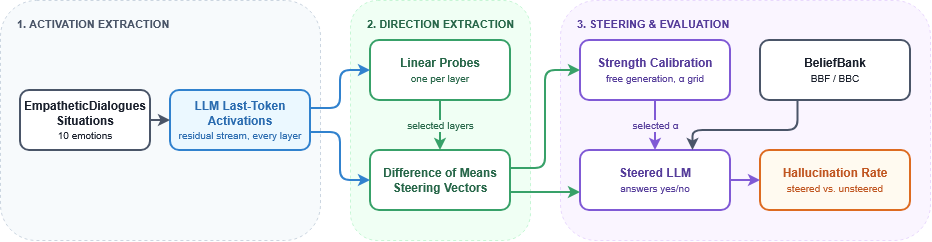
\includegraphics[width=1.0\linewidth]{images/pipeline.png}
  \caption{Overview of the pipeline.}
  \label{fig:pipelne}
\end{figure}



\subsection{Data preparation}
\label{sec:methods_data}
The EmpatheticDialogues data, originally split into training, validation, and testing, was merged, and the first 473 situations were selected for each emotion. This is the number of situations of the least frequent emotion, so that all emotions have the same number of situations. The texts in the dataset were cleaned: leading and trailing whitespace was stripped, and missing values, duplicates and texts shorter than two words were removed. This resulted in a final dataset with between 471 and 473 situations per emotion and an average length between about 15 and 22 words, depending on the emotion. To select the steering layer, the data was sampled into two balanced sets: 50 training situations and 50 test situations per emotion. Similarly, two additional balanced sets were created for calculating the steering vectors: 350 situations for the calculation and 100 test situations to verify them. These two pairs of sets were sampled independently, so they may overlap.

For BBF and BBC, since every combination of model, layer and emotion had to be evaluated, using the full datasets would have been too expensive. A fixed sample of 1{,}000 statements was therefore extracted from each of BBF and BBC with a fixed seed. For BBF, after removing duplicate statements, 500 statements were sampled for each label (\textit{yes/no}). For BBC, however, 500 complete pairs were sampled so that the number of statements per label remains balanced and each statement appears alongside its negation. The selected subsets were used for all models, allowing comparisons of the results obtained for the same statements.

\begin{table}[h]
  \centering
  \begin{tabular}{llrrl}
    \toprule
    Dataset & Use & Original & After cleaning & Samples used \\
    \midrule
    EmpatheticDialogues & layer selection & 473 / emotion & 471--473 / emotion & 50 train + 50 test / emotion \\
                        & steering vectors &               &                    & 350 train + 100 test / emotion \\
    BBF & evaluation & 27{,}416 & 27{,}414 & 1{,}000 (500 yes, 500 no) \\
    BBC & evaluation & 24{,}956 & 24{,}956 & 1{,}000 (500 pairs) \\
    \bottomrule
  \end{tabular}
  \caption{Datasets used in this work and size of the samples drawn from them.}
  \label{tab:datasets}
\end{table}


\subsection{Activation extraction}
\label{sec:methods_extraction}
Emotion representations were extracted from the residual stream~\cite{elhage2021mathematical} of the three models, where activation steering is usually applied~\cite{turner2024steeract, panickssery2024steerllama2}. All previously cleaned situations were fed to each model as plain text, without chat templates or instructions, so that the activations depended solely on the content of the situations. For each situation $x$ and each layer $\ell$, the hidden state of the last token, $h_\ell(x) \in \mathbb{R}^d$, was stored, where $d$ is the hidden size of the model. The last token was chosen since the models are causal, so it is the only position that can attend to the entire text. For this reason, its representation is commonly used to represent the whole sentence~\cite{liu2024universal, fu2025tokenprepending}, and most of the input can be recovered from it~\cite{zhao2026rep2text}. The texts were processed in batches with left padding, so that the last position always corresponds to the last real token. Texts longer than 256 tokens would be truncated, although no situation reaches this length. For efficiency reasons, the activations of all situations were extracted only once per model and then reused both for layer selection and for the calculation of the steering vectors.


\subsection{Layer selection}
\label{sec:methods_selection}
Activation steering is based on the assumption that the concept to be steered is represented as a direction in the residual stream~\cite{park2024linearrep, turner2024steeract, panickssery2024steerllama2}. Therefore, one way to find the layers where this assumption holds is linear probing~\cite{alain2018understanding}: a linear classifier was used to classify emotions from the activations of a layer; consequently, if the classifier performs well on a layer, the emotions are linearly separable there.

For each layer $\ell$, a separate probe was trained on the activations $h_\ell(x)$ of the layer-selection split (50 training and 50 test situations per emotion). The probe consists of a single linear layer followed by a softmax over the ten emotions:
\begin{equation}
p(e \mid x) = \mathrm{softmax}\big(W_\ell\, \tilde h_\ell(x) + b_\ell\big)_e ,
\end{equation}
where $\tilde h_\ell(x)$ is the activation standardized with the mean and standard deviation of each feature, computed on the training set only. The probe was trained by minimizing the cross-entropy loss with an L2 penalty of $0.01$ on the $W_\ell$ weights. Adam was used as the optimizer with a learning rate of $10^{-3}$ for 1{,}000 epochs. The probes were evaluated on test situations using the macro-F1 metric, i.e., the average of the F1 scores of the ten emotions. The results of probes are reported in Section~\ref{sec:results}

Each probe yields a macro-F1 value that can be used to construct a curve extending across all layers of each model. Since one of the goals of this work is to compare the behaviour of the models at multiple depths, several candidate layers were selected from the curve, chosen at the local maxima of the macro-F1 in the region where it reaches its plateau and distributed across different depths. The last layers were excluded, since they are more specialized in predicting the next token~\cite{lad2025remarkable}, and among the remaining ones the layer with the highest macro-F1 was always included.

\subsection{Steering vectors}
\label{sec:methods_vectors}
At each layer selected in the previous step, a steering vector was calculated for each emotion using the difference of means (following CAA~\cite{panickssery2024steerllama2}). Since the dataset contains no neutral situations, the target emotion was used as the positive class and the other nine emotions as the negative class. For an emotion $e$ and a layer $\ell$, the vector is the difference between the mean activation of the situations of $e$ and the mean activation of all the other situations:
\begin{equation}
v_e^{\ell} = \frac{1}{|D_e|} \sum_{x \in D_e} h_\ell(x) \;-\; \frac{1}{|D_{\neg e}|} \sum_{x \in D_{\neg e}} h_\ell(x),
\end{equation}
where $D_e$ contains the 350 training situations of $e$ in the steering split and $D_{\neg e}$ the training situations of the other emotions. In this way, $v_e^{\ell}$ represents what distinguishes the current emotion $e$ from the other emotions, cancelling out what the two classes share.

During generation, the model was steered by adding the normalized vector $\hat v_e^{\ell} = v_e^{\ell} / \|v_e^{\ell}\|$ to the residual stream of a single layer, i.e., to the output of layer $\ell$, as in previous work on activation steering~\cite{turner2024steeract, panickssery2024steerllama2, chen2025personavectors}. The vector was added at every token position, both the prompt and the generated tokens:
\begin{equation}
h_\ell \leftarrow h_\ell + \alpha \, \bar n_\ell \, \hat v_e^{\ell},
\end{equation}
where $\bar n_\ell$ is the mean norm of the activations at layer $\ell$ over all 3{,}500 training situations of the steering split (350 per emotion), and $\alpha$ is the steering strength. A vector of fixed norm would have a different effect across layers because the norm of the residual stream increases with depth and also varies across models. For this reason, the vector is scaled by $\bar n_\ell$, making $\alpha$ a fraction of the typical activation size: the same value can then be compared across layers and models. For example, $\alpha = 0.5$ adds a vector with a norm equal to half the mean norm of the activations at the chosen layer.

Once the steering vectors had been computed, a check was performed on the test split of 100 situations per emotion. This check verifies that the vectors capture the emotions: the test situations were projected onto the ten normalized steering vectors, after subtracting the mean activation over the same 3{,}500 training situations. Each situation was assigned to the emotion with the highest projection. In this case, the macro-F1 score was also computed to verify whether the calculated directions represent the emotions of unseen texts. The results are reported in Section~\ref{sec:results_vectors}.

\subsection{Choice of the steering strength}
\label{sec:methods_strength}
The steering strength must be large enough to show emotion in the model's response, but not so large that it no longer generates coherent text. This balance varies from emotion to emotion and from layer to layer, so $\alpha$ was calibrated separately for each combination. The analysis of the texts generated for the steering strength selection was done through four neutral prompts that leave room for an emotional tone: \textit{``Write a short story about a man walking home from work.''}, \textit{``Describe a rainy afternoon in the city.''}, \textit{``Continue the story: When I opened the door, I''} and \textit{``Write a short story about a woman waiting at a train station.''}. The prompts were given with the chat template of each model, and responses were generated with greedy decoding, up to 100 new tokens. For each layer and emotion, $\alpha$ was increased from $0.2$ up to $1.5$ in steps of $0.1$. A value of $\alpha = 0$ corresponds to an unsteered response: these responses were also generated and kept as a reference.

The generated texts were read and evaluated manually based on two aspects. The first is whether the tone, events, or words express the target emotion. The second is whether the text is broken, that is, if it presents one of the following situations: repeated words, meaningless characters, reasoning instead of a response, or role breaks (e.g.\ offering condolences or advice, asking what the task is). Short introductions such as \textit{``Certainly! Here's a short story''} were not considered failures.

The steering strength for each layer and emotion was then set according to the following criterion. Let $\alpha_{\mathrm{break}}$ be the smallest value at which at least one of the four texts is broken. The selected strength is $\alpha_{\mathrm{break}} - 0.2$, i.e., two steps before the first failure, which leaves a margin of safety. If the emotion was not visible in most texts at the selected value, $\alpha_{\mathrm{break}} - 0.1$ was chosen instead. This value was kept even if the emotion was still not clearly visible. In this way, the selected value makes the emotion as visible as possible while keeping the text intact.

\subsection{Evaluation on BeliefBank}
\label{sec:methods_evaluation}
To evaluate the effects of steering on the models' factual knowledge and simple inferences, the models were asked the yes/no questions from the BBF and BBC samples (Section~\ref{sec:methods_data}). The answers were generated first without steering and then with each steering condition, that is, each combination of layer and emotion with the corresponding steering strength selected. For both types of questions, the same prompt was used, with \texttt{\{statement\}} replaced with the statement to be evaluated:
\begin{quote}
\small\raggedright\texttt{You'll be provided with a fact, and your task is to confirm or deny its truthfulness.
Just answer only with yes or no. Is the fact true? Fact: \{statement\} Answer:}
\end{quote}
Again, the prompt was formatted with the model's chat template, and the answer was generated with greedy decoding and a limit of 50 tokens. Unsteered responses, generated only once per model, represent the baseline for all steering conditions.

Even when indicated in the prompt, models do not always answer with a single ``yes'' or ``no'', especially under steering, where the model's residual stream is modified. Each response was then mapped to \textit{yes}, \textit{no}, or \textit{unknown} using an ordered set of string rules. First, the text was converted to lowercase, and Markdown symbols and quotation marks were removed; if the first word was ``yes'' or ``no'', it was taken as the response; otherwise, if only one of the two words appears in the first sentence, that answer was used. Otherwise, if the first sentence states that the fact is true (e.g.\ ``true'', ``correct'') or false (e.g.\ ``false'', ``not true'', ``incorrect''), the answer was mapped to \textit{yes} or \textit{no}, respectively; otherwise, the answer was mapped to \textit{unknown}. Although reasoning mode was disabled, Qwen3.8 sometimes still reasons before answering, so only the text after reasoning was considered, and any answers that were interrupted before its end were mapped to \textit{unknown}.

Each steering condition was compared to the baseline using the following metrics:
\begin{itemize}
  \item \textbf{Hallucination rate}: the percentage of answers that do not match the label, where \textit{unknown} answers are considered incorrect.
  \item \textbf{Yes rate}: the percentage of \textit{yes} answers. A strong shift from 50\% indicates that steering is moving the model toward a fixed answer.
  \item \textbf{Unknown rate}: the percentage of \textit{unknown} responses. This represents the frequency with which the model abandons the yes/no format.
\end{itemize}

\subsection{Experimental setup}
\label{sec:methods_setup}
The pipeline was implemented in Python. The PyTorch and Hugging Face \texttt{transformers} libraries were used, with \texttt{bitsandbytes} for 4-bit quantization and \texttt{scikit-learn} for evaluation metrics. The experiments on Qwen2.5 and Llama were run locally on an NVIDIA GeForce RTX 3050 GPU with 8\,GB of memory: quantization allowed the models to fit in the available memory. The experiments on Qwen3.8-27B were instead run on an NVIDIA A100 80\,GB GPU via the Modal cloud platform (\url{https://modal.com}).

For random operations such as sampling the data splits, defining the BeliefBank subsets and initializing the probes, the same seed (42) was used. Greedy decoding also makes text generation deterministic for a given prompt, so the results can be reproduced. Table~\ref{tab:hyper_pipeline} summarizes the main hyperparameters of the pipeline.

\begin{table}[h]
  \centering
  \begin{tabular}{lll}
    \toprule
    Step & Hyperparameter & Value \\
    \midrule
    Data & seed & 42 \\
    Activation extraction & max input length & 256 tokens \\
    Linear probe & optimizer, learning rate & Adam, $10^{-3}$ \\
                 & epochs, L2 penalty & 1{,}000, $0.01$ \\
    Steering vectors & training / test situations & 350 / 100 per emotion \\
    Strength calibration & prompts, max new tokens & 4, 100 \\
                         & $\alpha$ grid step & $0.1$ \\
    Evaluation & questions per subset, max new tokens & 1{,}000, 50 \\
    Generation & decoding & greedy \\
    \bottomrule
  \end{tabular}
  \caption{Main hyperparameters of the pipeline.}
  \label{tab:hyper_pipeline}
\end{table}

\section{Results}
\label{sec:results}

\subsection{Layer selection}
\label{sec:results_layer}
Figure~\ref{fig:probing} shows the macro-F1 score of the probes at each layer as a function of the relative depth. The macro-F1 increases rapidly, exceeding $0.50$ around 20--35\% depth in the three models. A plateau is then reached that lasts until the last layer: $0.55$--$0.61$ for Qwen2.5, which keeps improving until layer 25; $0.55$--$0.58$ for Llama, almost flat from layer 14 onward; and $0.50$--$0.58$ for Qwen3.8, with a dip around layers 43--48. In all models, in the last layers, the score decreases slightly or remains stable.

The plateau is almost flat, so the differences between the best layers are minimal: in Qwen3.8, the three highest values (layers 63, 39 and 27) differ by less than $0.001$. The layers were therefore chosen to cover different depths: 14, 20, and 25 for Qwen2.5; 17, 24, and 27 for Llama; and 27, 39, 50, and 54 for Qwen3.8, i.e., approximately 40--90\% of the depth. The Qwen3.8 layer with the highest value is layer 63, which was excluded as one of the last layers (Section~\ref{sec:methods_selection}).

\begin{figure}[t]
  \centering
  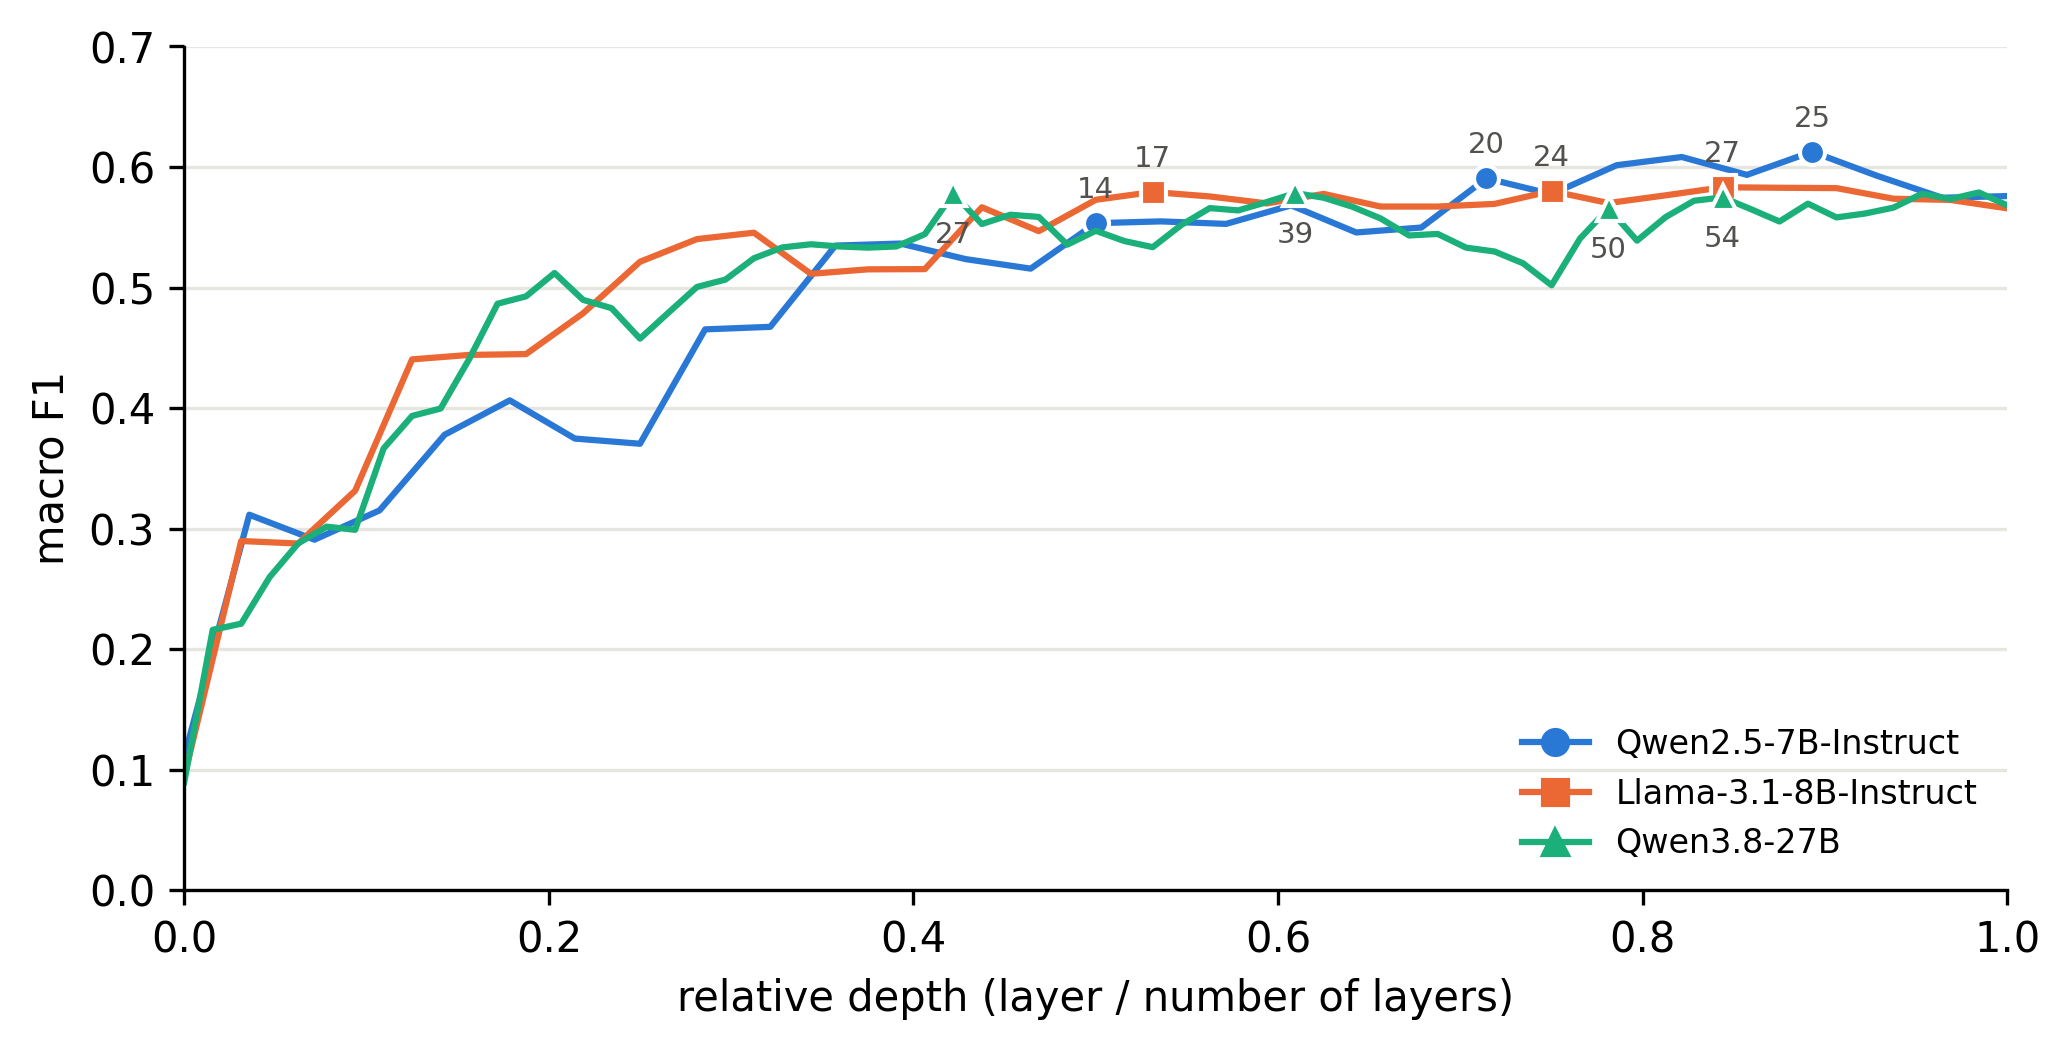
\includegraphics[width=0.9\linewidth]{images/probing_macro_f1.png}
  \caption{Macro-F1 of the linear probes at each layer, as a function of the relative depth (layer / number of layers). The markers indicate the layers selected for steering.}
  \label{fig:probing}
\end{figure}

\subsection{Steering vectors}
\label{sec:results_vectors}
As described in Section~\ref{sec:methods_vectors}, one of the checks on the computed steering vectors is to project the test situations onto them. The macro-F1 scores obtained from this classification are reported in Table~\ref{tab:projection}, along with the macro-F1 scores of the probes at the same layer. Even though the vectors are simple differences of means and no classifier was trained, their macro-F1 ($0.50$--$0.61$) is well above chance ($0.10$) and very close to that of the probes: apart from layer 54 of Qwen3.8, the values differ by at most $0.05$, and the projection is slightly better than the probe in Llama, at layer 14 of Qwen2.5, and in the first two layers of Qwen3.8. It is slightly worse in the other layers of Qwen2.5; the gap is larger only at layers 50 and 54 of Qwen3.8. The comparison between the probes and the projections is only indicative, since the two methods were evaluated on different test sets.

\begin{table}[t]
  \centering
  \begin{tabular}{lrrr}
    \toprule
    Model & Layer & Projection macro-F1 & Probe macro-F1 \\
    \midrule
    Qwen2.5 & 14 & 0.57 & 0.55 \\
            & 20 & 0.57 & 0.59 \\
            & 25 & 0.58 & 0.61 \\
    \midrule
    Llama   & 17 & 0.61 & 0.58 \\
            & 24 & 0.60 & 0.58 \\
            & 27 & 0.60 & 0.58 \\
    \midrule
    Qwen3.8 & 27 & 0.61 & 0.58 \\
            & 39 & 0.60 & 0.58 \\
            & 50 & 0.52 & 0.57 \\
            & 54 & 0.50 & 0.57 \\
    \bottomrule
  \end{tabular}
  \caption{Macro-F1 of the classification by projection onto the steering vectors on the test situations of the steering split, compared with the macro-F1 of the linear probe at the same layer.}
  \label{tab:projection}
\end{table}

\subsection{Steering strength}
\label{sec:results_strength}
Table~\ref{tab:alphas} shows the steering strengths selected for each emotion and layer. In all models, the text breaks at lower strengths in the shallowest selected layers, while the deepest one is among the most tolerant: the mean $\alpha$ ranges from $0.66$ to $0.76$ in Qwen2.5, from $0.61$ to $0.80$ in Llama, and from $0.49$ to $0.84$ in Qwen3.8. The variability between emotions depends on the layer: at layer 17 of Llama, almost every emotion has the same strength ($0.6$), while at layer 14 of Qwen2.5, the values range from $0.3$ to $1.0$. At this layer, \textit{sad} and \textit{devastated} break the text even at low strengths.

Table~\ref{tab:examples} shows how the generated text changes as $\alpha$ increases for a prompt steered toward \textit{anxious} at layer 17 of Llama. Without steering, a neutral scene of a woman waiting for a train is described. At the selected strength ($\alpha = 0.6$), the same prompt leads to a different story, focusing on the woman's nervousness. With $\alpha = 1.0$, the text turns into a stream of confused thoughts, and with $\alpha = 1.2$, it breaks down completely, repeating the same phrase over and over.

The depth of the steered layer also affects the way the emotion appears. Steering in intermediate layers tends to modify the content of the story, while in deeper layers, the text often remains similar to the unsteered one and the emotion is expressed only through a few inserted words. Table~\ref{tab:depth} shows an example for \textit{ashamed} in Llama: at layer 17 a scene is described with empty streets and people going out of necessity or shame, while at layer 27 the text is almost identical to the one without steering except for a few words.

\begin{table}[h!]
  \centering
  \small
  \begin{tabular}{l ccc ccc cccc}
    \toprule
    & \multicolumn{3}{c}{Qwen2.5} & \multicolumn{3}{c}{Llama} & \multicolumn{4}{c}{Qwen3.8} \\
    \cmidrule(lr){2-4} \cmidrule(lr){5-7} \cmidrule(lr){8-11}
    Emotion & 14 & 20 & 25 & 17 & 24 & 27 & 27 & 39 & 50 & 54 \\
    \midrule
    afraid     & 0.7 & 0.8 & 0.8 & 0.6 & 0.9 & 1.0 & 0.4 & 0.6 & 0.8 & 1.0 \\
    angry      & 0.7 & 0.7 & 0.8 & 0.6 & 0.6 & 0.8 & 0.5 & 0.7 & 0.6 & 0.9 \\
    annoyed    & 0.6 & 0.6 & 0.9 & 0.6 & 0.8 & 0.8 & 0.7 & 0.7 & 0.6 & 0.8 \\
    anxious    & 0.4 & 0.8 & 0.8 & 0.6 & 0.9 & 0.8 & 0.4 & 0.6 & 0.5 & 0.9 \\
    ashamed    & 0.8 & 0.8 & 0.7 & 0.6 & 0.7 & 0.7 & 0.5 & 0.9 & 0.7 & 0.6 \\
    content    & 1.0 & 0.9 & 0.7 & 0.6 & 0.9 & 0.9 & 0.5 & 0.6 & 0.6 & 0.9 \\
    devastated & 0.4 & 0.8 & 0.7 & 0.6 & 0.8 & 0.8 & 0.5 & 0.6 & 0.6 & 0.7 \\
    joyful     & 0.8 & 0.8 & 0.8 & 0.6 & 0.6 & 0.7 & 0.4 & 0.5 & 0.9 & 0.9 \\
    sad        & 0.3 & 0.6 & 0.6 & 0.7 & 0.8 & 0.9 & 0.4 & 0.6 & 0.5 & 0.9 \\
    trusting   & 0.9 & 0.8 & 0.7 & 0.6 & 0.7 & 0.6 & 0.6 & 0.7 & 0.5 & 0.8 \\
    \midrule
    mean       & 0.66 & 0.76 & 0.75 & 0.61 & 0.77 & 0.80 & 0.49 & 0.65 & 0.63 & 0.84 \\
    \bottomrule
  \end{tabular}
  \caption{Steering strength $\alpha$ selected for each emotion and layer, with the mean over the ten emotions.}
  \label{tab:alphas}
\end{table}

\begin{table}[h!]
  \centering
  \small
  \begin{tabular}{cp{0.85\linewidth}}
    \toprule
    $\alpha$ & Generated text \\
    \midrule
    0.0 & \textit{It was a drizzly summer evening, and the train station was dimly lit, the only sound being the soft hum of the fluorescent lights above. Emma stood by the large glass windows [\dots]} \\
    0.6 & \textit{The Waiting Hour. As the clock ticks away, Emily stands in front of the large, whiteboard displaying the train schedules. She takes a deep breath, trying to calm her nerves. The familiar feeling of uncertainty is creeping in [\dots]} \\
    1.0 & \textit{The Waiting Hour. What is the time?...? The thought keeps racing through Sarah's mind as she sits in the waiting area at the Clouty Station. [\dots] The time is not about the general aspect of the unknown, but about the [\dots]} \\
    1.2 & \textit{The Unknown Sign on the Door. What is the most common aspect of the unknown?? For many, it is the unknown about the unknown. For most, it is the unknown about the unknown about the unknown. For many, it is the unknown about the unknown about the unknown about the unknown [\dots]} \\
    \bottomrule
  \end{tabular}
  \caption{Text generated by Llama for the prompt ``Write a short story about a woman waiting at a train station.'', steered towards \textit{anxious} at layer 17. The selected strength for this condition is $\alpha = 0.6$.}
  \label{tab:examples}
\end{table}

\begin{table}[h!]
  \centering
  \small
  \begin{tabular}{lp{0.8\linewidth}}
    \toprule
    Condition & Generated text \\
    \midrule
    Baseline & \textit{A rainy afternoon in the city is a unique and captivating experience. The sky is a deep, foreboding grey, with thick clouds that seem to swallow the sun whole. The air is cool and damp [\dots]} \\
    Layer 17 ($\alpha = 0.6$) & \textit{A rainy afternoon in the city is a scene that is both gloomy and intriguing. [\dots] The city's streets, once bustling with pedestrians, are now empty, save for a few brave individuals who, out of necessity or shame, walked out of the building [\dots]} \\
    Layer 27 ($\alpha = 0.7$) & \textit{A rainy afternoon in the city is a unique and captivating experience. The sky is a deep, \textbf{remorseless} grey, with thick, \textbf{heavy} clouds that seem to \textbf{weigh down upon} the urban landscape. The air is cool and damp [\dots]} \\
    \bottomrule
  \end{tabular}
  \caption{Text generated by Llama for the prompt ``Describe a rainy afternoon in the city.'' without steering and steered towards \textit{ashamed} at layers 17 and 27. In bold, the words that differ from the baseline.}
  \label{tab:depth}
\end{table}

\subsection{Effect on factual knowledge}
\label{sec:results_knowledge}
Without steering, the three models have a low hallucination rate on BBF statements (4--7\%), with a balanced yes rate (46--54\%). On BBC, however, the hallucination rate is much higher (39--53\%), close to chance, and the two Qwen models answer ``no'' to most statements (yes rates of 10\% for Qwen2.5 and 14\% for Qwen3.8); Llama is more balanced, with a yes rate of 56\%. For the two Qwen models, the BBC hallucination rate reflects a bias towards ``no'' more than the ability to reason about constraints. Therefore, BBF is the main benchmark to measure the damage that steering causes to factual knowledge, while on BBC the shift in the yes rate is more informative than the hallucination rate.

The effect of steering on BBF depends primarily on the depth at which it is applied (Figure~\ref{fig:bbf_accuracy}). The greatest damage appears in the intermediate layers, at a depth of approximately 50--61\% (layer 14 of Qwen2.5, 17 of Llama, and 39 of Qwen3.8). Here, the average hallucination rate across the ten emotions increases by 20--37 points. Beyond the intermediate layers, the damage decreases, and in the deepest selected layers (84--89\% depth), the hallucination rate remains very close to the baseline for almost all emotions. On BBC, the hallucination rate changes much less (Figure~\ref{fig:bbc_accuracy}), as a model already close to chance cannot get much worse; the largest increases occur where unknown answers are frequent.

Figure~\ref{fig:yes_rate} shows the yes rate for each layer and emotion. At intermediate layers, positive emotions (\textit{content}, \textit{joyful}, \textit{trusting}) push the model towards ``yes''. In the two Qwen models, most negative emotions tend to produce ``no'' answers, while in Llama, almost all emotions lead to ``yes'' answers at layer 17. In the deepest layers, the BBF yes rate remains stable at around 50\%, the only exception being \textit{joyful} in Qwen3.8, with a yes rate of 91\% at layer 54.

The unknown rate is zero in the baselines and in every combination of Qwen2.5. An unknown rate well above zero occurs only at layer 24 of Llama (\textit{sad} and \textit{anxious} yield 28\% and 22\% unknown responses on BBF and up to 64\% on BBC) and at layer 27 of Qwen3.8 (\textit{trusting} yields 42\% on BBF and up to 81\% on BBC).

These results are consistent with the texts generated in Section~\ref{sec:results_strength}: in the intermediate layers, steering changes both the content of the stories and the answers to factual questions, while in the deeper layers, where the emotion appears only through a few added words, the answers stay almost intact.

\begin{figure}[p]
  \centering
  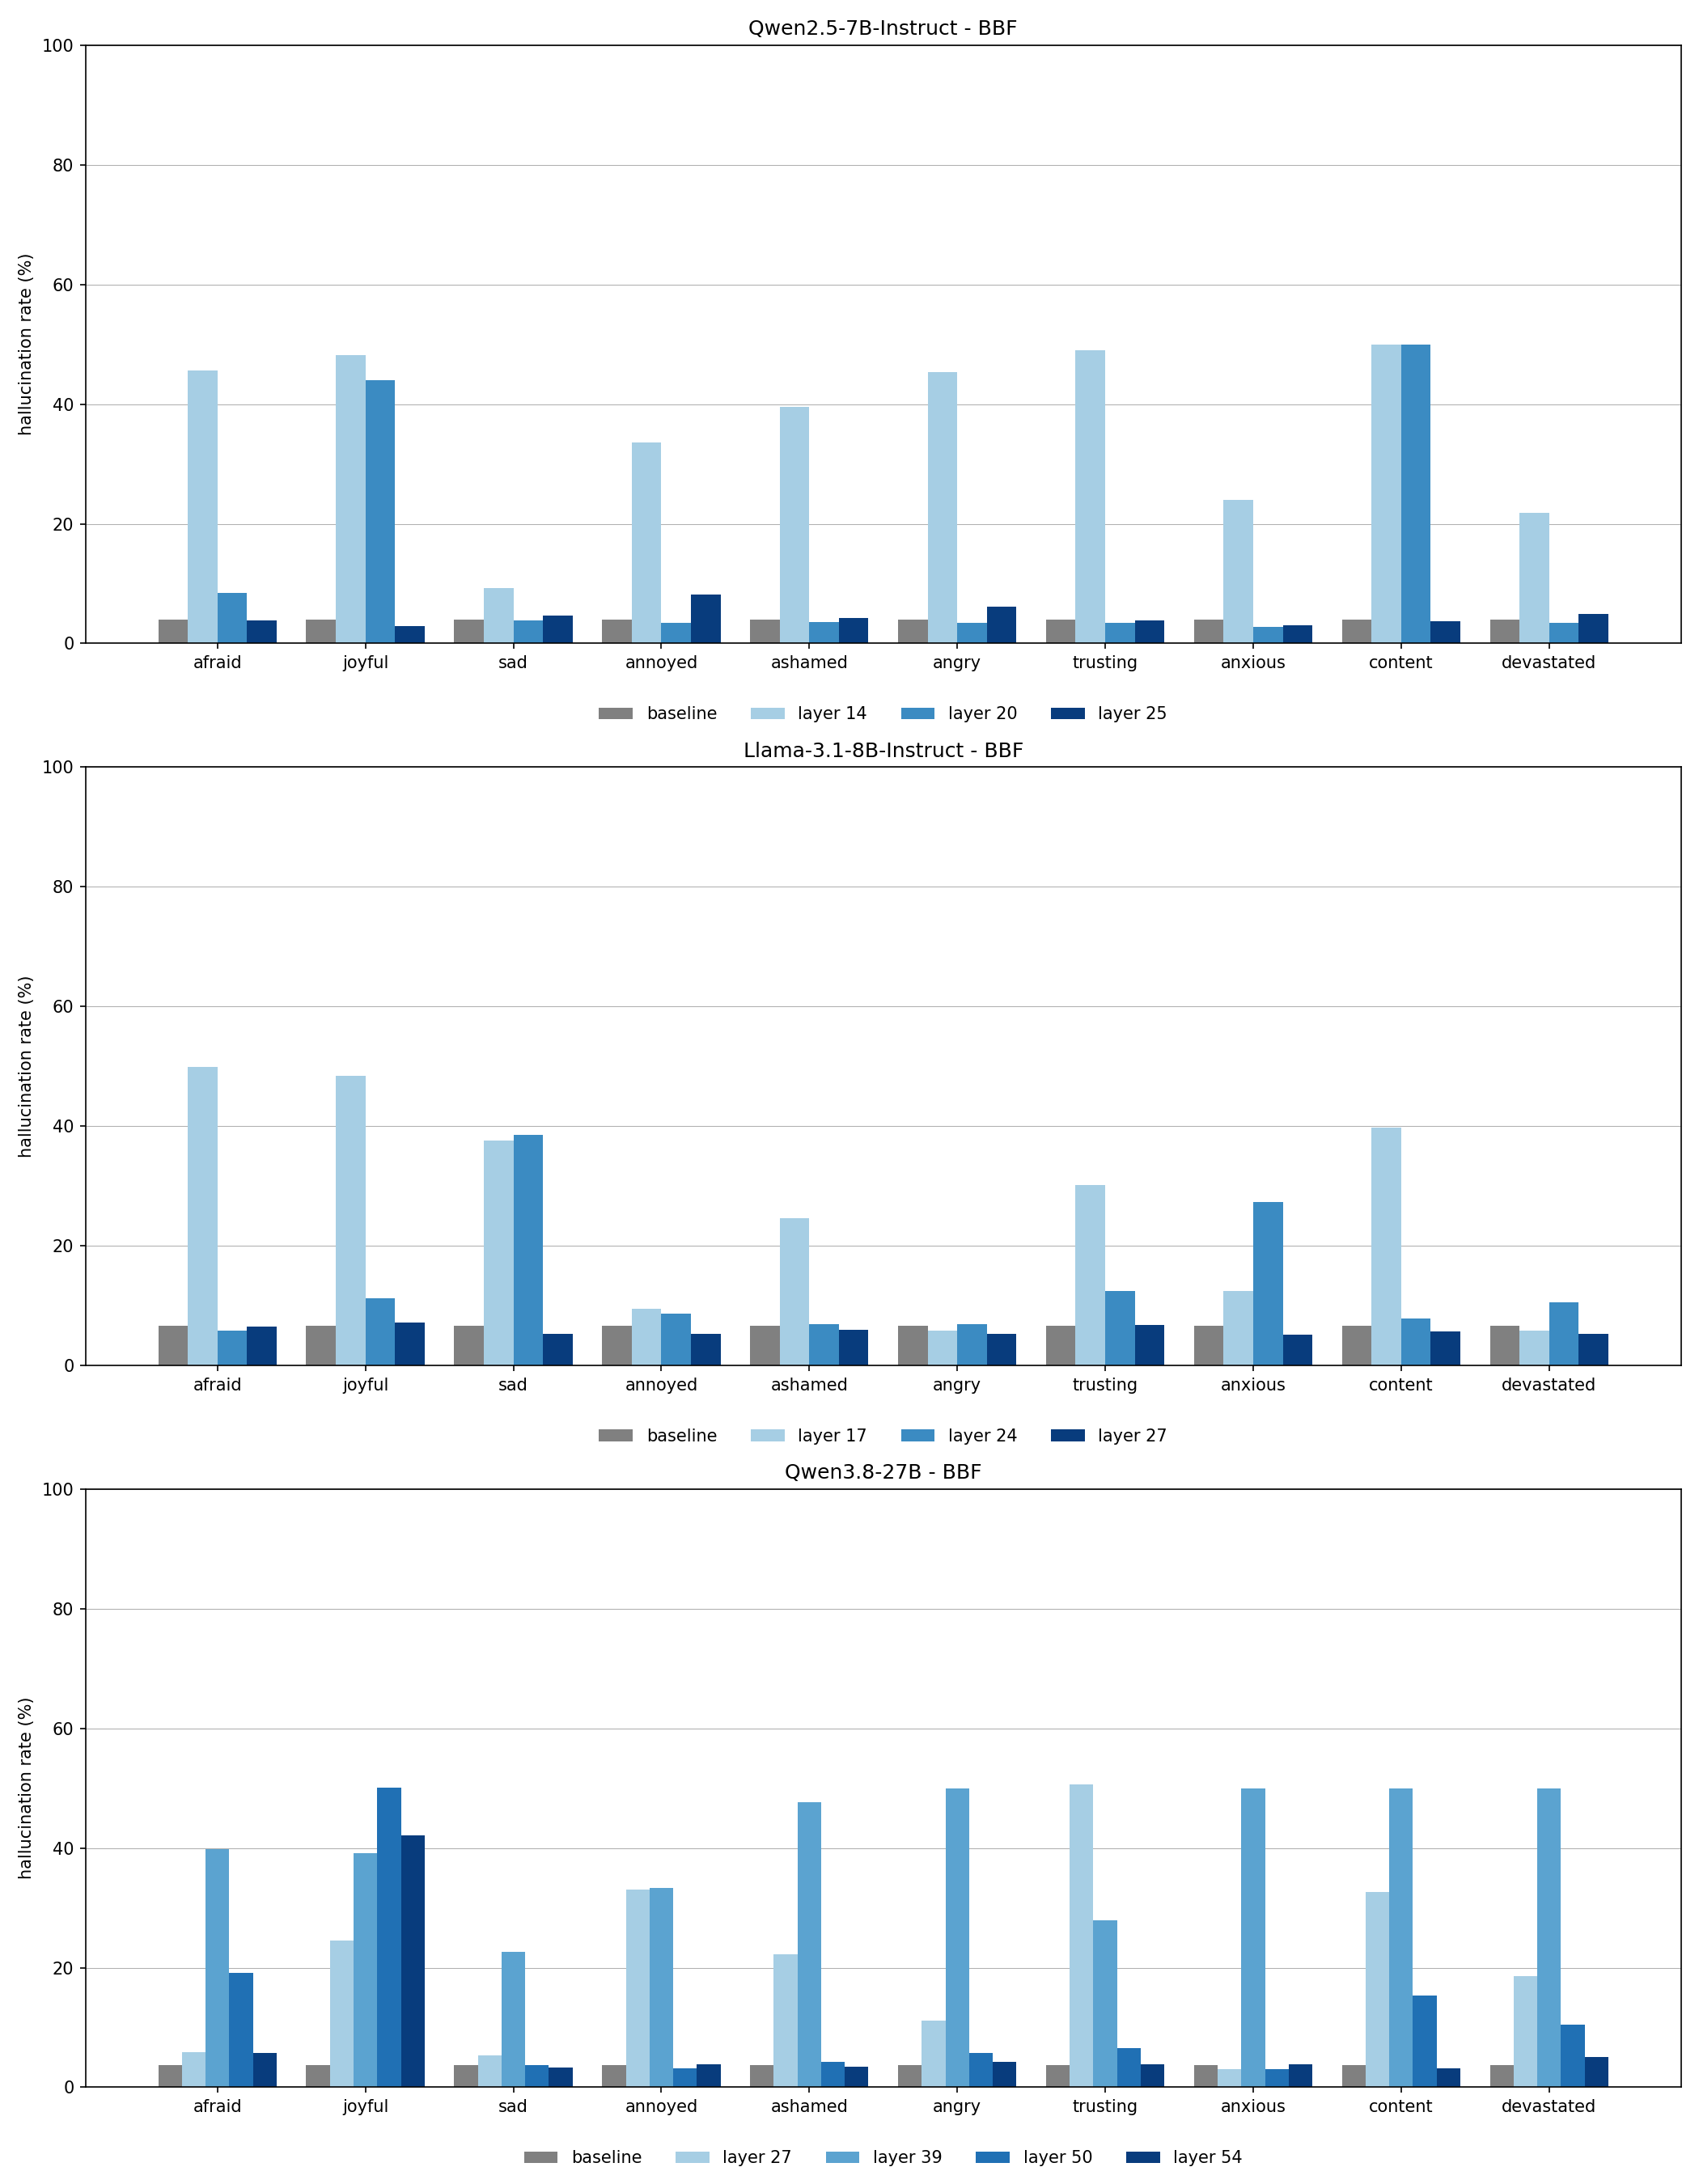
\includegraphics[width=\linewidth]{bbf_hallucination_all.png}
  \caption{Hallucination rate on BBF for each emotion, without steering (gray) and with steering at each selected layer.}
  \label{fig:bbf_accuracy}
\end{figure}

\begin{figure}[p]
  \centering
  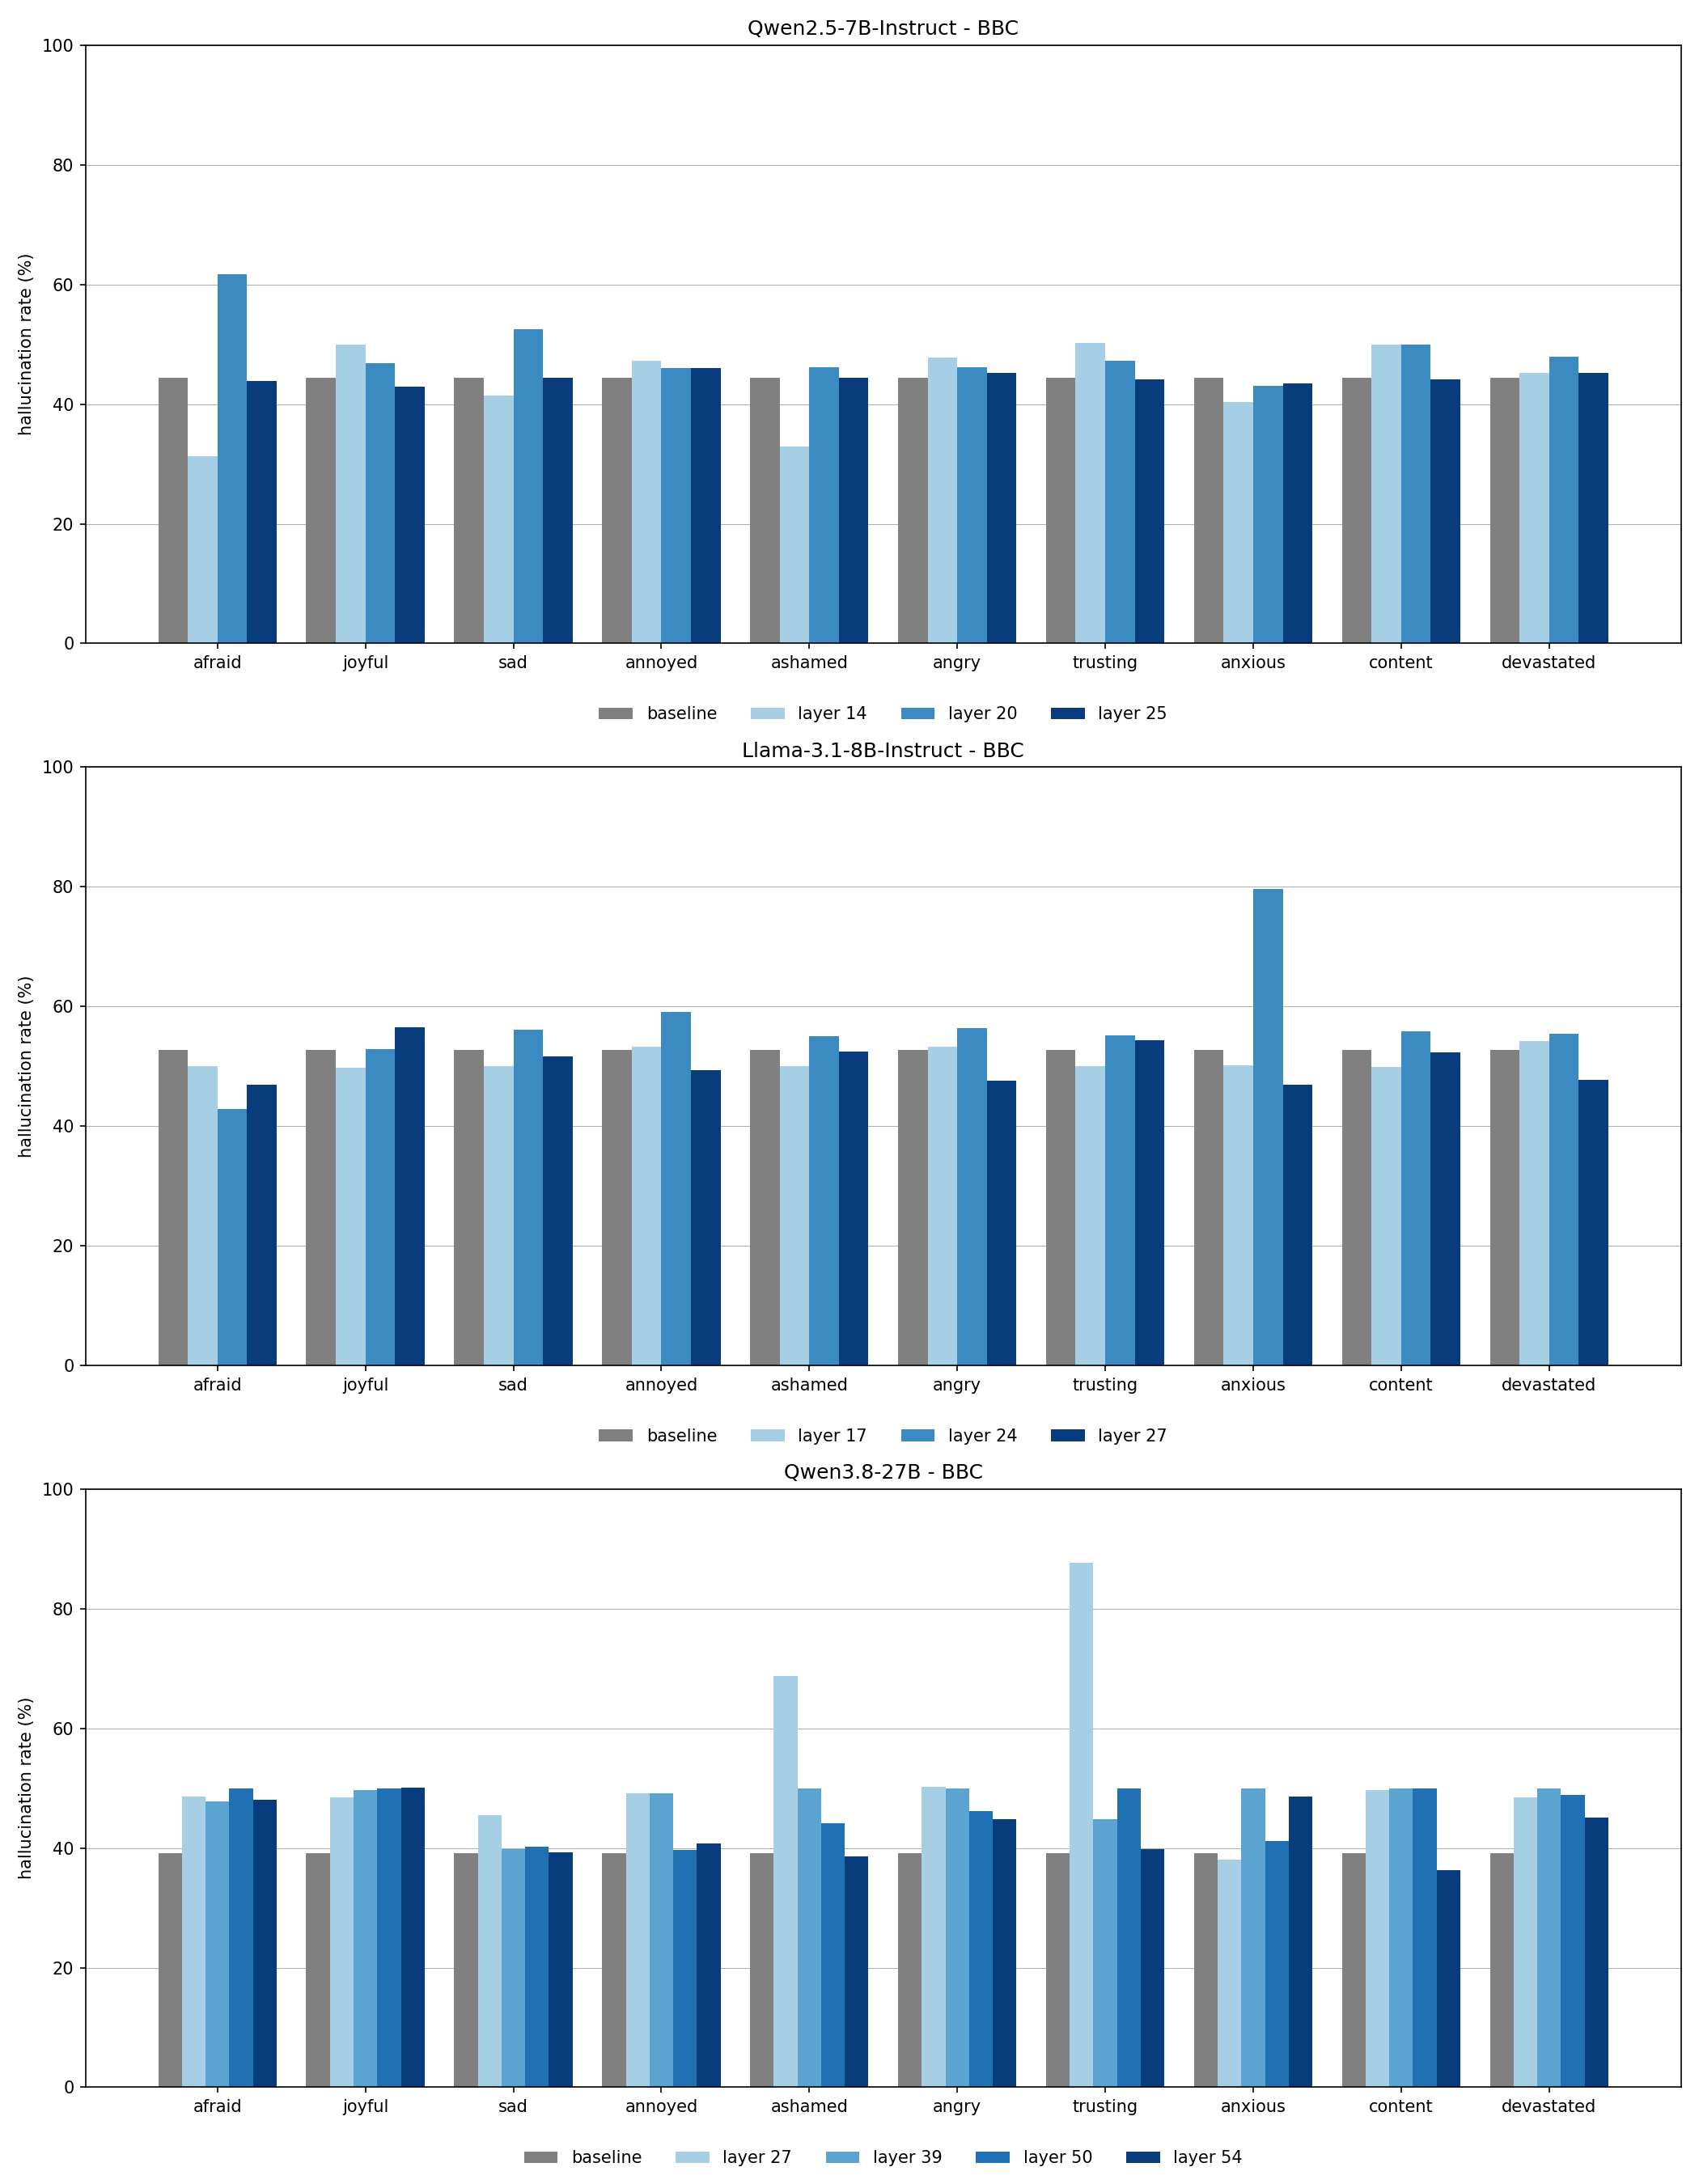
\includegraphics[width=\linewidth]{bbc_hallucination_all.png}
  \caption{Hallucination rate on BBC for each emotion, without steering (gray) and with steering at each selected layer.}
  \label{fig:bbc_accuracy}
\end{figure}

\begin{figure}[t]
  \centering
  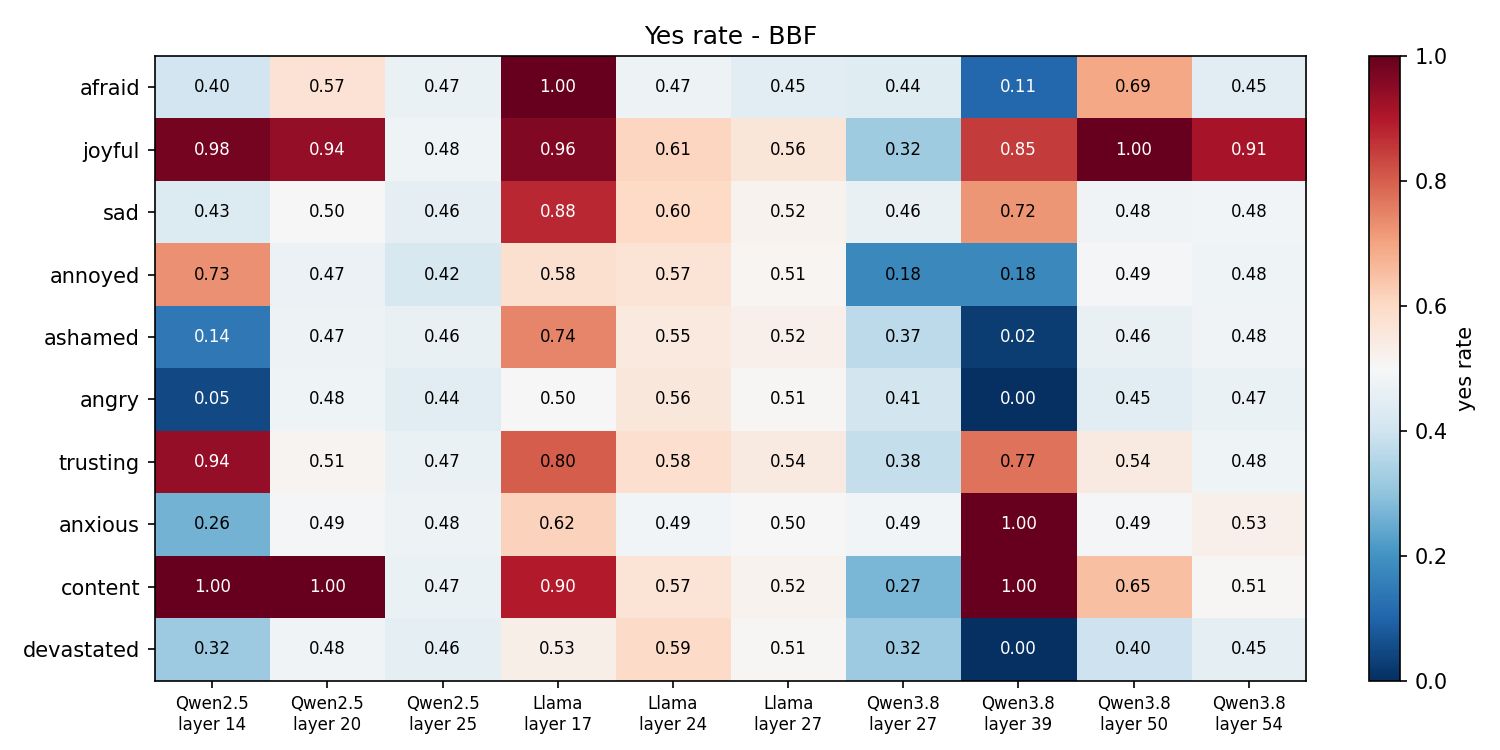
\includegraphics[width=\linewidth]{bbf_yes_rate.png}\\[4pt]
  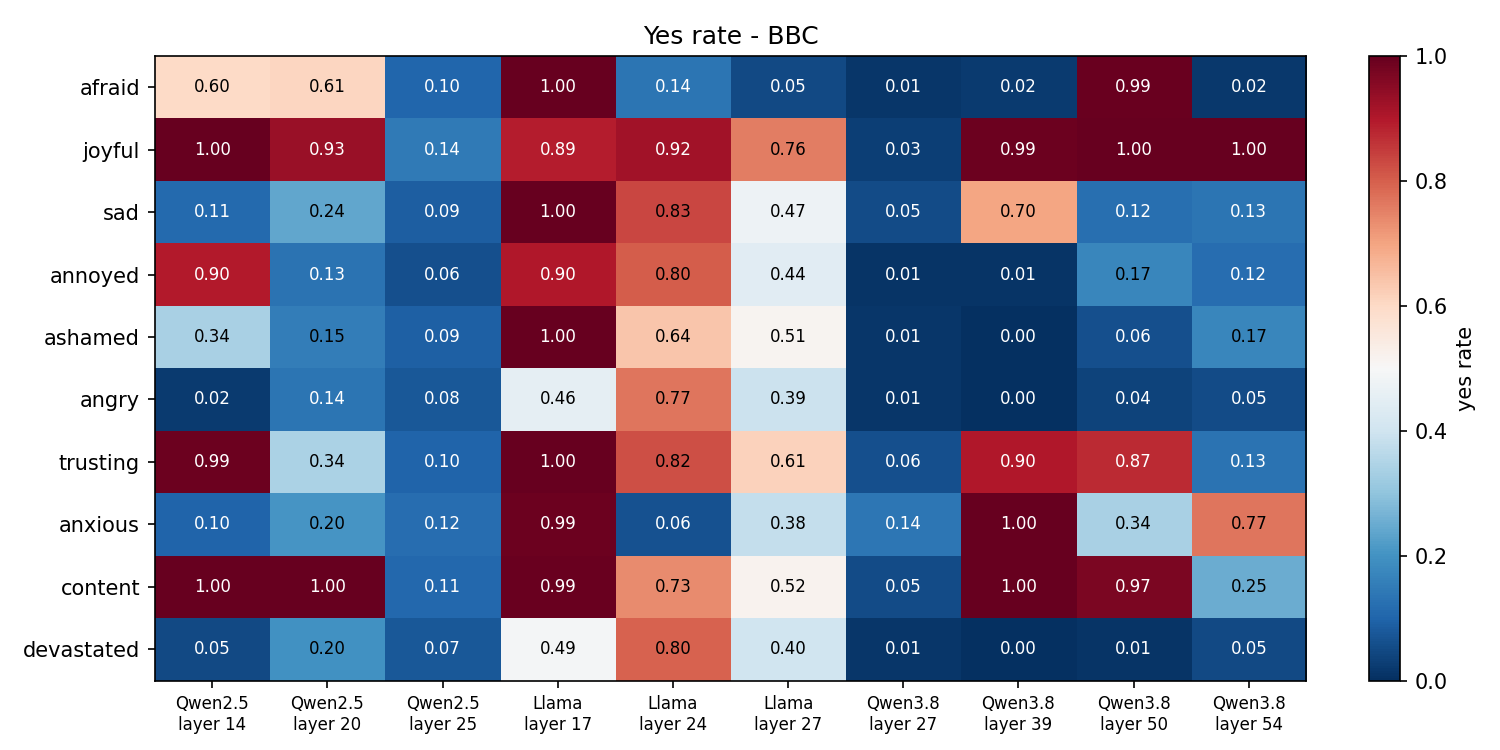
\includegraphics[width=\linewidth]{bbc_yes_rate.png}
  \caption{Yes rate of each emotion at each model and layer, on BBF (top) and BBC (bottom). Blue cells correspond to models answering mostly ``no'', red cells to models answering mostly ``yes''.}
  \label{fig:yes_rate}
\end{figure}

\newpage
\section{Conclusion}
This work studied how a model's answers to factual and logical questions change when it is steered towards an emotion, and how this depends on the depth of the steered layer. Linear probes showed that emotions become linearly separable starting from a specific point in the network, remaining so until the last layer. The steering vectors, although simple differences of means, separated the emotions almost as well as the probes. With a strength calibrated on free generation for each layer and emotion, the effect on factual knowledge and simple inferences turned out to depend mainly on depth: steering at intermediate layers led to a large increase in the hallucination rate, often reducing answers to a constant ``yes'' or ``no'', while at deeper layers, the hallucination rate remained close to the baseline. The generated texts, however, show that where the answers are preserved the emotion is more superficial: in deeper layers it appears only through a few added words, while in intermediate layers it changes the content of the text.

This study also has several limitations. Steering strengths were selected by manually reading the texts generated from only four prompts, and the evaluation was done by a single annotator, so the criterion is partly subjective. In addition, the selected strength is fixed for each layer and emotion, whereas it could be adapted dynamically, for example to each input or activation~\cite{wang2024act}. Regarding the BBC dataset, without steering, the models are already close to chance, and this limits what the dataset can reveal about knowledge of relationships between concepts. Moreover, only factual and simple logical errors were evaluated: other types of hallucinations were not analysed, although benchmarks such as HaluEval~\cite{li2023halueval} could be used for this purpose. A single prompt and greedy decoding were used, and the two smaller models were quantized to 4 bits. Finally, only a few layers per model were tested, so the depth at which the damage disappears is only approximately known.

Possible future work includes replacing manual strength calibration with automatic measures of emotion visibility and text comprehensibility. Other steering methods could also be explored to make the emotion clearly visible without harming the model's factual knowledge.
\bibliographystyle{unsrt}  
\bibliography{references}

\end{document}
